% This is just some examples example of how to implement a figure with a caption.
% It should be run standalone so you can use it for testing. It won't matter if you break it as it's not
% included in the main template anywhere.


\documentclass[11pt]{article}
\usepackage{import}
\usepackage{graphicx}
\usepackage{caption}
\usepackage{tabularray,xcolor}
\usepackage{lipsum}
\definecolor{NiceGray}{RGB}{248,248,248}

\begin{document}

%insert a figure.

\begin{figure}[h]
    \noindent
        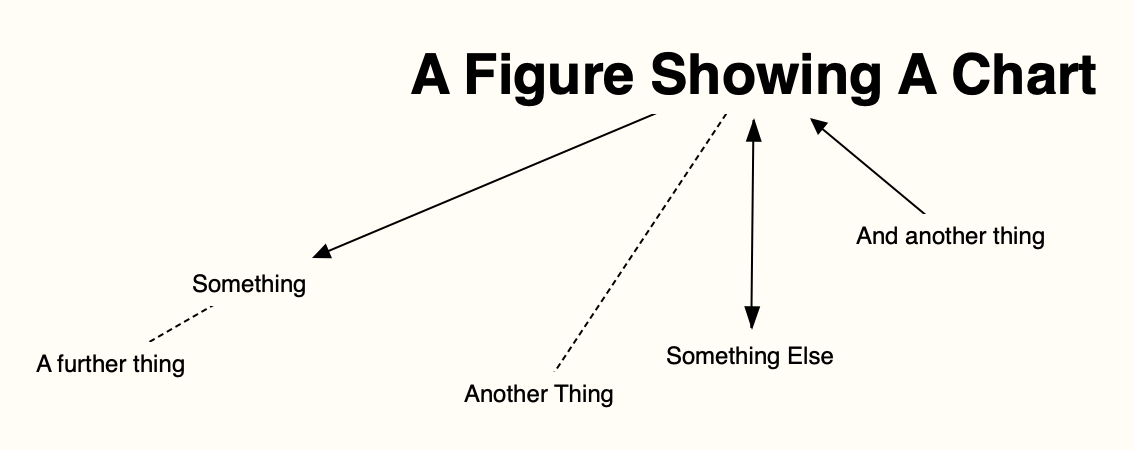
\includegraphics[scale=0.6, width=\textwidth]{images/FigureofTest}
        \caption{A chart with some text underneath it that i would like to break over lines and make sure it's long enough}
        \label{fig:chartex}
\end{figure}


\lipsum[2]


% This is a nested table that shows you can achieve some complex layouts.
% Wraping things inside a basic table allows greater control over where  you put things on the page.
% I use the tabularray package to allow things like tall tables that will continue across pages.

\begin{table}[htp]
    \centering

    \begin{talltblr}
        [
         caption = {A weird nested table because for some reason I needed one},
         entry = {Serial Square},
         label = {tblr:serial-square}
        ]
        {
         rows = {2em, rowsep = 2pt},
         %columns = {2em, colsep = 2pt},
         %hspan = minimal,
         row{1} = {bg = NiceGray, 0.2em, rowsep=0.5pt},
         %width = {.8\linewidth},
         colspec = {X[1,l] | X[1,l]  X[1,l]  X[1,l] X[1,l] X[1,l] },
        }
     % this makes row one a table within the row
     \SetCell[c=6]{c,f}{
        \begin{tblr}
            {
             hspan =  minimal,
             baseline = f,
             width = \linewidth,
             colspec = {X [1,r] X[1,r] X[1,r] X[1,r] X[1,r] X[1,r]},
            }
            \SetCell{r}{\scriptsize ${-2}$} &
            \SetCell{r}{\scriptsize ${+3}$} &
            \SetCell{r}{\scriptsize ${-3}$} &
            \SetCell{r}{\scriptsize ${+4}$} &
            \SetCell{r}{\scriptsize ${+4}$} &
        \end{tblr}}
        & 2-6 & 3-6 & 4-6 & 5-6 & 6 % you need to specify the rest of the cell contents
     \\

        Table Row 1 & 1 & 4 & 1 & 5 & 9 \\
        Table Row 2 & 2 & 3 & 3 & 4 & 4 \\
        Table Row 3 & 1 & 2 & 4 & 5 & 6 \\
        Table Row 4 & 2 & 3 & 4 & 6 & 6 \\
        Table Row 5 & 4 & 6 & 5 & 6 & 8 \\
        Table Row 6 & 2 & 1 & 5 & 1 & 3 \\
    \end{talltblr}
\end{table}

\paragraph*{New Paragraph}

text to reference Figure \ref{fig:chartex} \newline
% text to reference Table \ref{tblr:serial-square}
\end{document}
